\documentclass[11pt]{article}
\usepackage[letterpaper,margin=0.82in,headheight=15pt]{geometry}
\usepackage{amsmath,amssymb,mathtools}
\usepackage{booktabs,array}
\usepackage{graphicx}
\usepackage{xcolor}
\usepackage{float}
\usepackage{caption}
\usepackage{subcaption}
\usepackage{enumitem}
\usepackage{listings}
\usepackage{fancyhdr}
\usepackage[hidelinks]{hyperref}
\usepackage{microtype}

\definecolor{navy}{HTML}{153B5B}
\definecolor{bluegray}{HTML}{EEF3F7}
\definecolor{codegreen}{HTML}{276749}
\definecolor{codepurple}{HTML}{6B46C1}
\definecolor{codegray}{HTML}{5F6B73}

\pagestyle{fancy}
\fancyhf{}
\lhead{IE 598: Reinforcement Learning and Learning-Based Control}
\rhead{Homework 1}
\cfoot{\thepage}
\renewcommand{\headrulewidth}{0.4pt}

\setlength{\parindent}{0pt}
\setlength{\parskip}{5pt}
\setlist[itemize]{topsep=3pt,itemsep=2pt}
\setlist[enumerate]{topsep=3pt,itemsep=2pt}
\captionsetup{font=small,labelfont=bf}

\lstset{
  language=Python,
  basicstyle=\ttfamily\small,
  keywordstyle=\color{navy}\bfseries,
  commentstyle=\color{codegreen},
  stringstyle=\color{codepurple},
  numbers=left,
  numberstyle=\scriptsize\color{codegray},
  stepnumber=1,
  numbersep=8pt,
  frame=single,
  rulecolor=\color{navy!35},
  backgroundcolor=\color{bluegray!60},
  breaklines=true,
  breakatwhitespace=false,
  columns=fullflexible,
  keepspaces=true,
  showstringspaces=false,
  aboveskip=7pt,
  belowskip=7pt
}

\newcommand{\E}{\mathbb{E}}
\newcommand{\R}{\mathbb{R}}
\newcommand{\argmin}{\operatorname*{arg\,min}}
\newcommand{\argmax}{\operatorname*{arg\,max}}
\newcommand{\answerbox}[1]{%
  \begin{center}
  \fcolorbox{navy}{bluegray}{\parbox{0.9\linewidth}{#1}}
  \end{center}}

\begin{document}

\begin{titlepage}
  \centering
  \vspace*{1.35in}
  {\color{navy}\rule{\textwidth}{1.4pt}}\\[0.34in]
  {\Huge\bfseries Homework 1: Final Submission\par}
  \vspace{0.22in}
  {\Large IE 598: Reinforcement Learning and Learning-Based Control\par}
  \vspace{0.34in}
  {\color{navy}\rule{\textwidth}{1.4pt}}\\[0.65in]
  {\large Dynamic programming, partial observation, and convex interpolation\par}
  \vspace{0.32in}
  {\Large Prachit Gupta\par}
  \vspace{0.10in}
  {\large NetID: \texttt{prachit2}\par}
  \vfill
  \begin{minipage}{0.84\textwidth}
    \small
    \textbf{AI-use note.} AI assistance was used to typeset this report from the
    author's verified handwritten solutions and Markdown files and to help phrase
    intuitive explanations. The complete project and source materials are available at
    \href{https://github.com/prachitgupta/RL_LearningBasedControl}%
    {\texttt{github.com/prachitgupta/RL\_LearningBasedControl}}.
  \end{minipage}
  \par
  \vspace{0.35in}
  {\large September 18, 2026\par}
\end{titlepage}

\pagenumbering{roman}
\tableofcontents
\clearpage
\pagenumbering{arabic}

\section{Question 1: Inventory Control}

The disturbance and one-period inventory cost are
\[
w_t=\begin{cases}
1,&\text{with probability }1/2,\\
3,&\text{with probability }1/2,
\end{cases}
\qquad
c(x)=\begin{cases}
x,&x\ge 0,\\
-1000x,&x<0.
\end{cases}
\]
The stage and terminal costs are
\[
g_t(m_t,u_t)=c(m_t)+2u_t,\qquad g_2(m_2)=c(m_2).
\]

\subsection{Terminal stage}

At $t=N=2$,
\[
J_2^*(m_2)=g_2(m_2)=c(m_2)
=\begin{cases}
m_2,&m_2\ge 0,\\
-1000m_2,&m_2<0.
\end{cases}
\]

\subsection{Stage $t=1$}

Backward dynamic programming gives
\begin{align*}
J_1^*(m_1)
&=\min_{u_1}\E_{w_1}\!\left[c(m_1)+2u_1
   +J_2^*(m_1+u_1-w_1)\right]\\
&=c(m_1)+\min_{u_1}F_1(u_1),
\end{align*}
where
\begin{align*}
F_1(u_1)
&=2u_1+\frac12J_2^*(m_1+u_1-1)
          +\frac12J_2^*(m_1+u_1-3)\\[2mm]
&=\begin{cases}
-998u_1-1000m_1+2000,
    &m_1+u_1<1,\\[1mm]
\dfrac{-995u_1-999m_1+2999}{2},
    &1\le m_1+u_1<3,\\[3mm]
3u_1+m_1-2,
    &m_1+u_1\ge 3.
\end{cases}
\end{align*}
The slopes of the three pieces are $-998$, $-995/2$, and $3$. Therefore, the minimum occurs at the second breakpoint:
\[
u_1^*=3-m_1.
\]
Substitution gives
\[
F_1(u_1^*)=3(3-m_1)+m_1-2=7-2m_1,
\]
and hence
\answerbox{$\displaystyle J_1^*(m_1)=c(m_1)+7-2m_1,\qquad
\mu_1^*(m_1)=3-m_1.$}

Equivalently,
\[
J_1^*(m)=
\begin{cases}
7-1002m,&m<0,\\
7-m,&m\ge 0.
\end{cases}
\]

\subsection{Stage $t=0$}

Continue the same recursion:
\begin{align*}
J_0^*(m_0)
&=\min_{u_0}\E_{w_0}\!\left[c(m_0)+2u_0
   +J_1^*(m_0+u_0-w_0)\right]\\
&=c(m_0)+\min_{u_0}F_0(u_0),
\end{align*}
where
\begin{align*}
F_0(u_0)
&=2u_0+\frac12J_1^*(m_0+u_0-1)
          +\frac12J_1^*(m_0+u_0-3)\\[2mm]
&=\begin{cases}
-1000u_0-1002m_0+2011,
    &m_0+u_0<1,\\[1mm]
\dfrac{-999u_0-1003m_0+3021}{2},
    &1\le m_0+u_0<3,\\[3mm]
u_0-m_0+9,
    &m_0+u_0\ge 3.
\end{cases}
\end{align*}
The slopes are $-1000$, $-999/2$, and $1$, so the minimum again occurs at the second breakpoint:
\[
u_0^*=3-m_0.
\]
At this control,
\[
F_0(u_0^*)=(3-m_0)-m_0+9=12-2m_0.
\]
Therefore,
\answerbox{$\displaystyle J_0^*(m_0)=c(m_0)+12-2m_0,\qquad
\mu_0^*(m_0)=3-m_0.$}
In particular,
\answerbox{$\displaystyle J_0^*(0)=c(0)+12=12.$}

\begin{figure}[H]
  \centering
  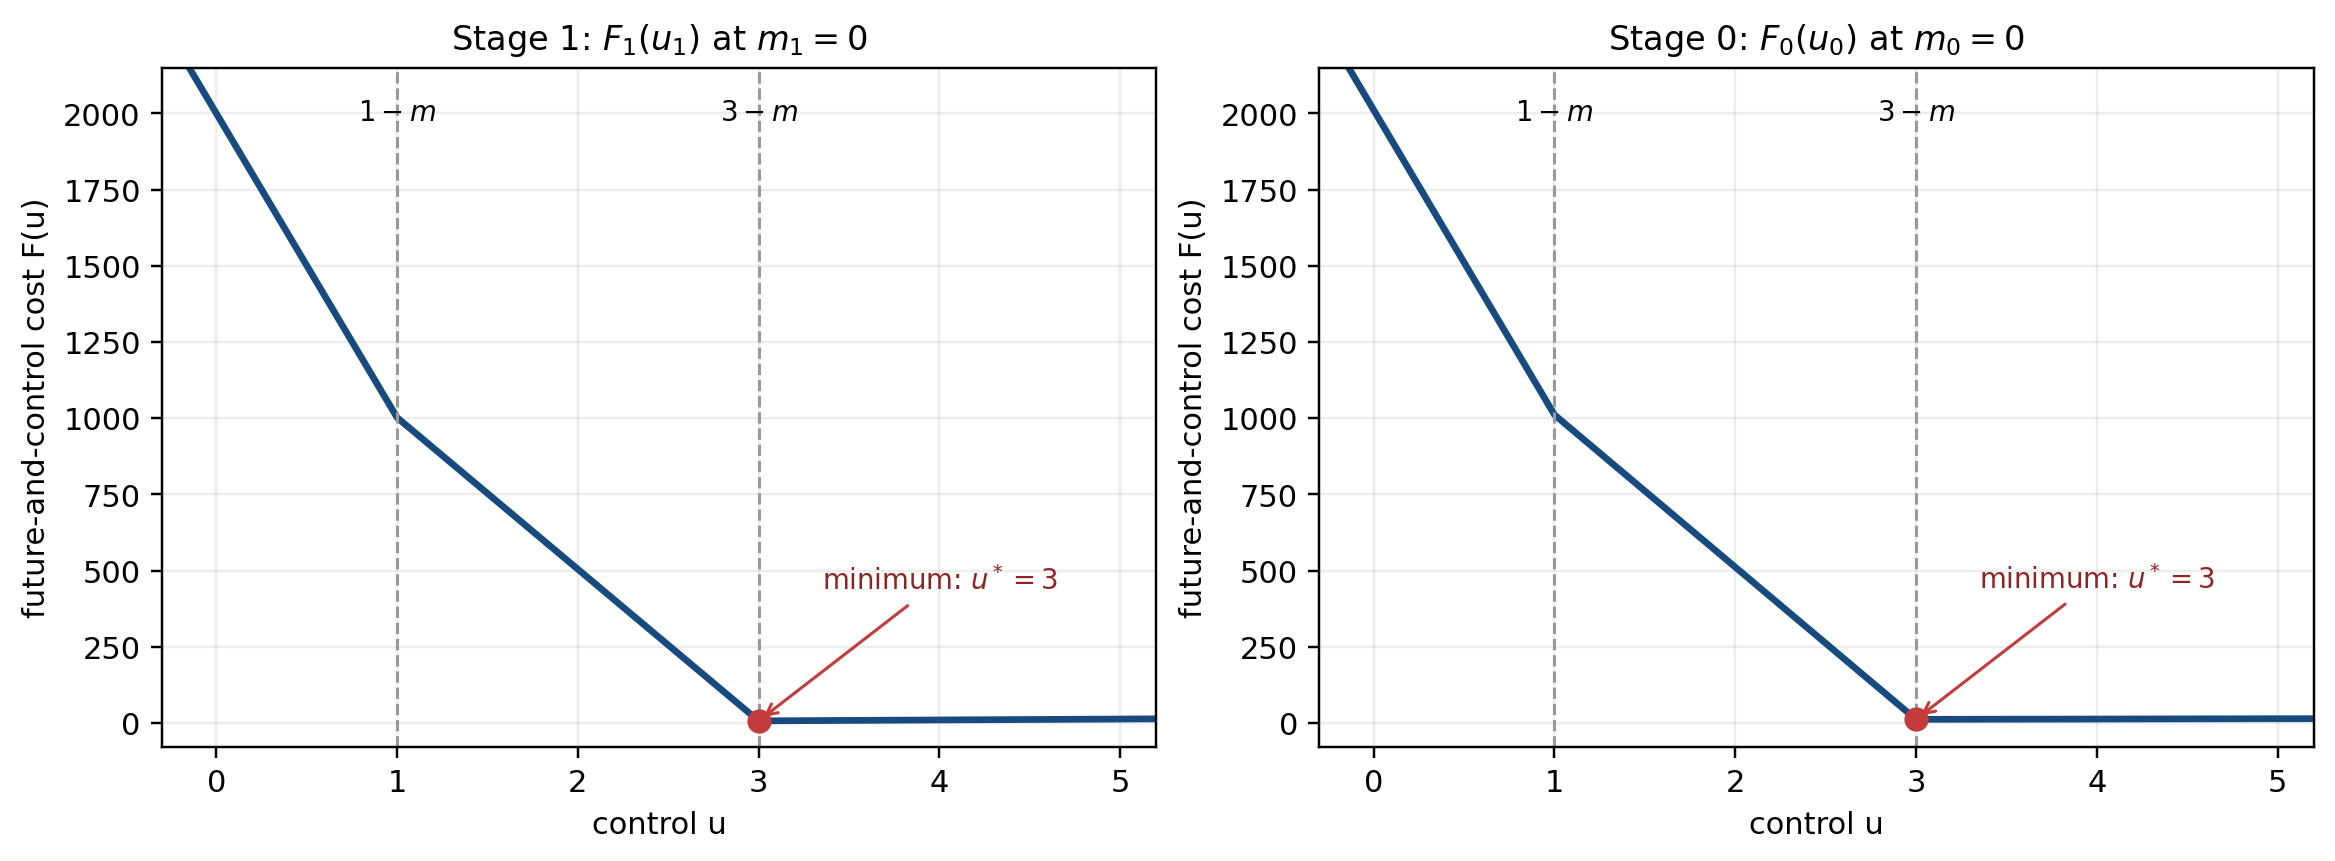
\includegraphics[width=0.98\textwidth]{report_figures/q1_piecewise_plots.png}
  \caption{Piecewise-linear functions minimized at stages 1 and 0, shown for $m_1=m_0=0$. The dashed lines mark the two breakpoints. The same geometry shifts horizontally by $-m_t$ for a general inventory state.}
\end{figure}

\clearpage
\section{Question 2: GridWorld}

The implementation uses the given $6\times 6$ grid, three obstacle cells, absorbing goal $G=(5,5)$, horizon $N=15$, transition probabilities in \texttt{Basic\_Functions.py}, and the supplied random seed $24$. Only \texttt{MDP.py}, \texttt{POMDP.py}, and \texttt{MAP.py} were edited.

\subsection{1(a): Finite-horizon dynamic programming}

The terminal values are initialized as $J_N^*(x)=c_N(x)$. For $t=N-1,\ldots,0$, the code evaluates
\[
J_t^*(x)=\min_{u\in\mathcal U}
\left[c(x,u)+\sum_{x'}P(x'\mid x,u)J_{t+1}^*(x')\right].
\]
The completed portion of \texttt{MDP.py} is:
\begin{lstlisting}
J_opt[N, :] = bf.terminal_costs

for t in range(N - 1, -1, -1):
    for s_index in range(S):
        J_opt[t, s_index] = min([
            stage_cost_c(s_index, a)
            + sum([
                transition_prob[a, s_index, s_next]
                * J_opt[t + 1, s_next]
                for s_next in range(S)
            ])
            for a in range(A)
        ])
\end{lstlisting}

\subsection{1(b): Heat maps of $J_0^*$ and $J_6^*$}

\begin{figure}[H]
  \centering
  \begin{subfigure}[t]{0.49\textwidth}
    \centering
    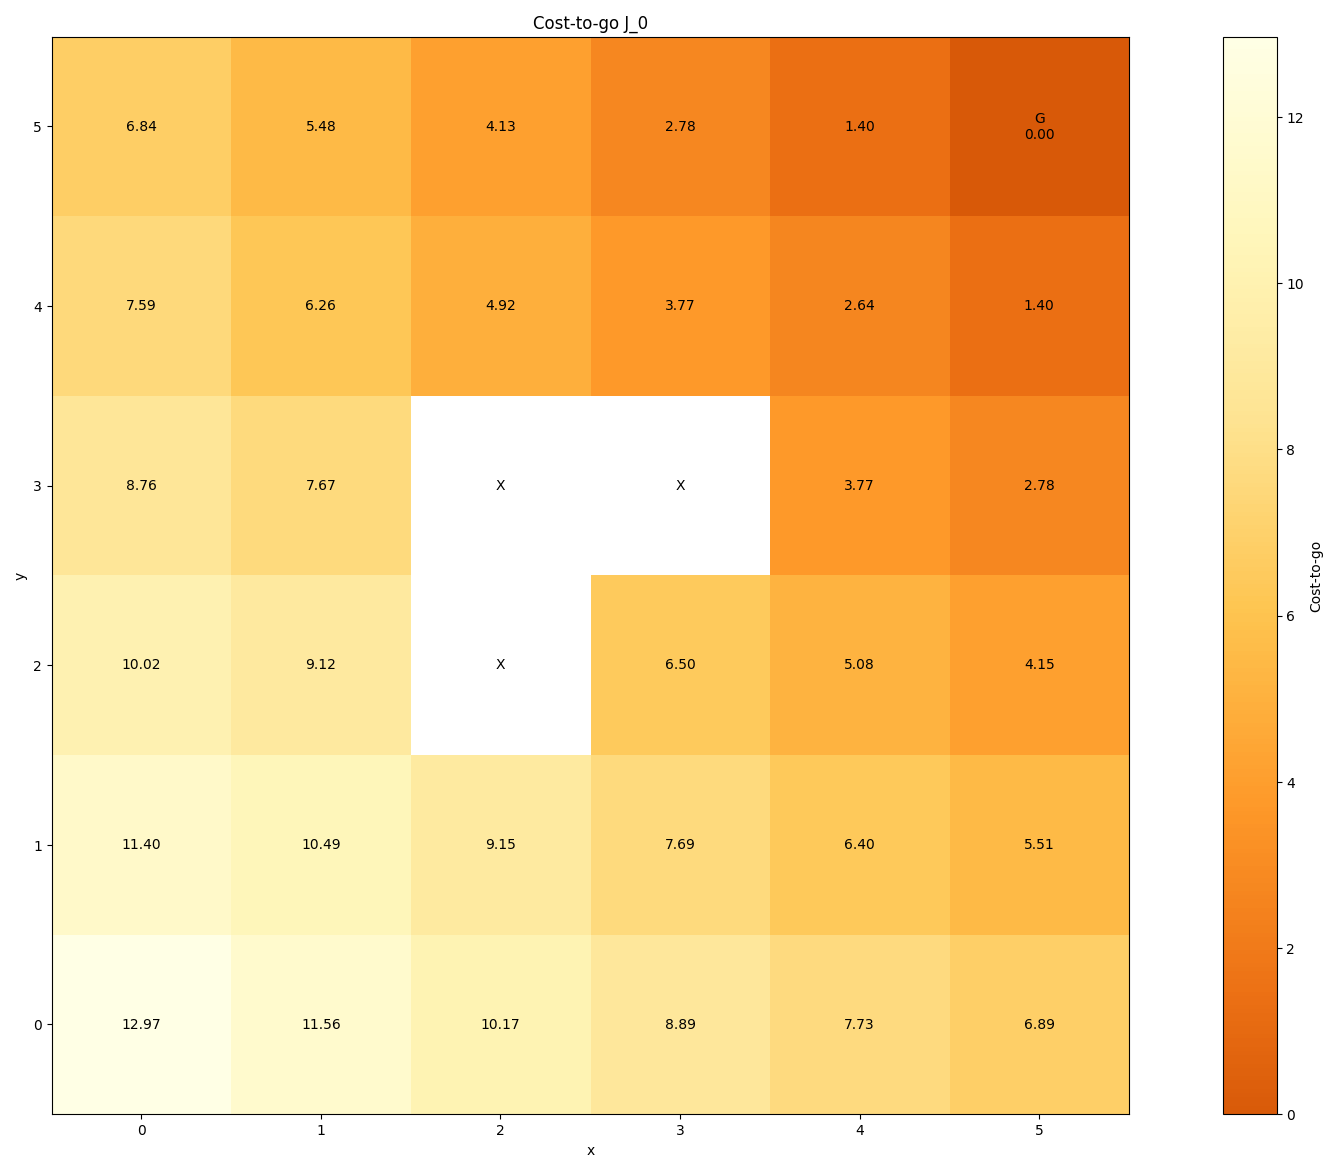
\includegraphics[width=\textwidth]{report_figures/j0_part1.png}
    \caption{$J_0^*$}
  \end{subfigure}\hfill
  \begin{subfigure}[t]{0.49\textwidth}
    \centering
    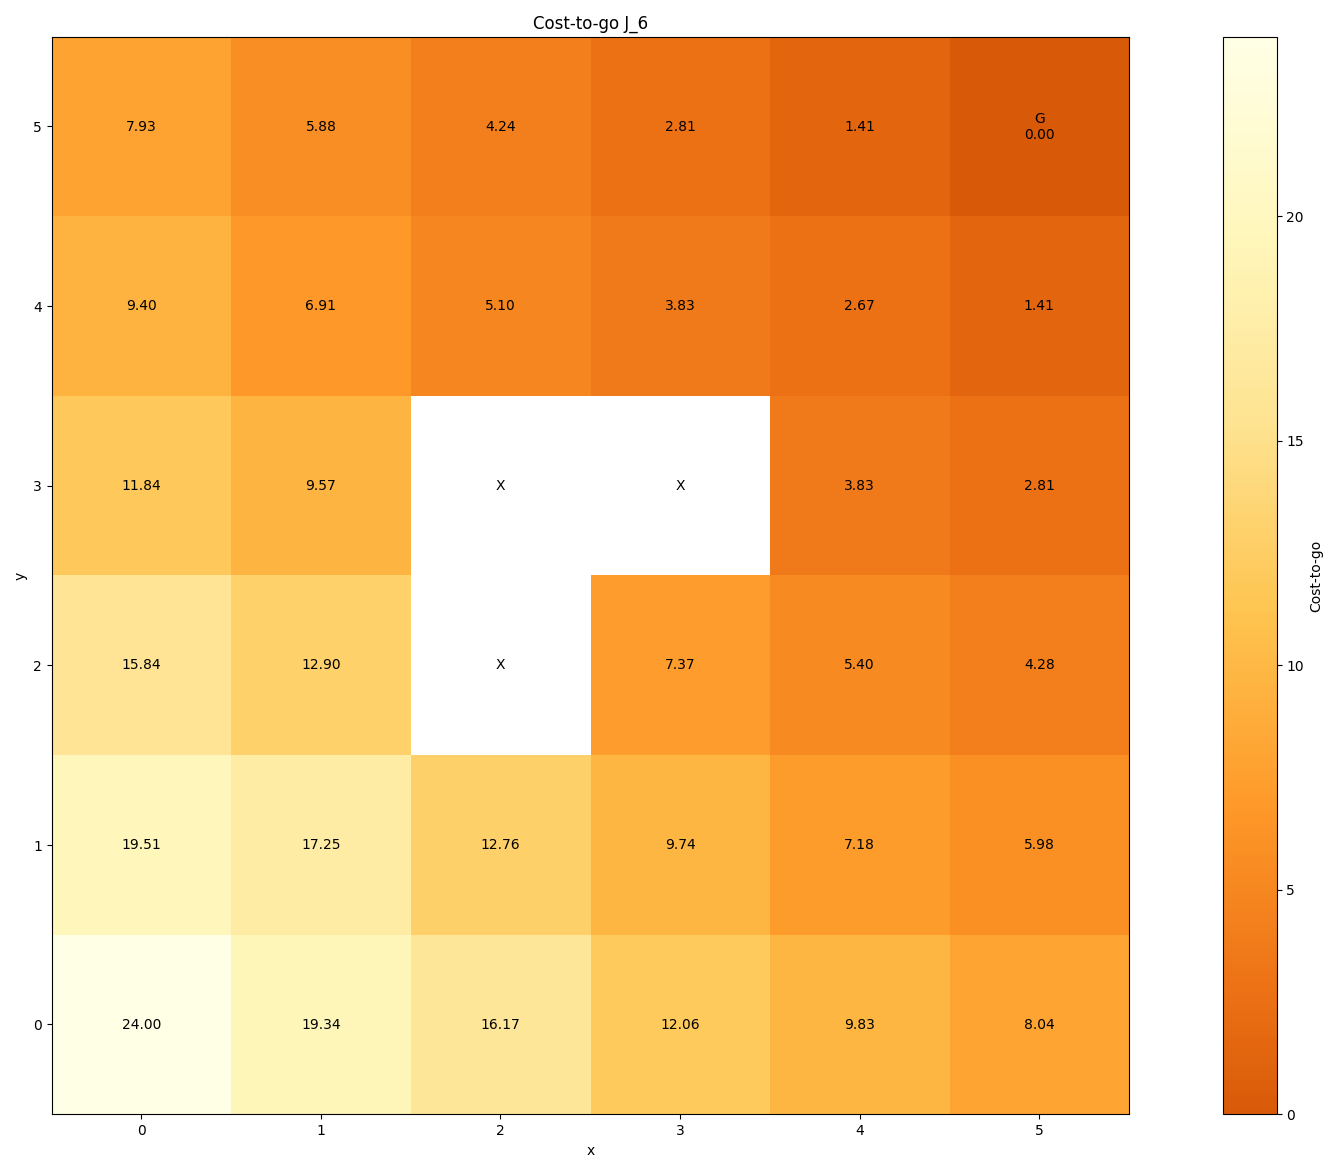
\includegraphics[width=\textwidth]{report_figures/j6_part1.png}
    \caption{$J_6^*$}
  \end{subfigure}
  \caption{Optimal finite-horizon cost-to-go heat maps. White cells marked $X$ are obstacles and $G$ is the absorbing goal.}
\end{figure}

\subsection{1(c): Comparing $J_0^*$ and $J_6^*$}

As evident in the heat maps, for the same state $x$, $J_6^*(x)$ is generally larger than $J_0^*(x)$. At $t=6$, the robot has fewer remaining time steps before the terminal horizon, so it has fewer opportunities to reach the goal. Hence, it has a higher probability of remaining outside the goal at $t=N$ and incurring the terminal penalty of 15. In contrast, starting from $t=0$ gives the robot more time to reach the absorbing goal, after which the stage cost is zero.

Although the Bellman equation adds the current stage cost to the expected future cost, this does not imply that the cost-to-go must increase as we move backward in time. The future-cost term also changes because an earlier starting time provides more opportunities to reach the goal and avoid the relatively large terminal penalty. In this case, that benefit outweighs the extra stage costs, so $J_0^*(x)$ is generally smaller than $J_6^*(x)$.

\subsection{2(a): Exact Bayesian belief update}

For an action $u_t$ and new observation $y_{t+1}$, define
\[
\operatorname{Term1}(x')=P(y_{t+1}\mid x')
\sum_x P(x'\mid x,u_t)b_t(x).
\]
Then
\[
b_{t+1}(x')=\frac{\operatorname{Term1}(x')}
{\sum_{\tilde x}\operatorname{Term1}(\tilde x)}.
\]
The completed portion of \texttt{POMDP.py} is:
\begin{lstlisting}
term1 = np.zeros(S)

for s_next in range(S):
    for s in range(S):
        term1[s_next] += (
            belief[s]
            * transition_prob[action_index, s, s_next]
            * observation_prob[s_next, observation_index]
        )

updated_belief = np.zeros(S)
if term1.sum() > 0:
    updated_belief = term1 / term1.sum()

return updated_belief
\end{lstlisting}

\subsection{2(b): Belief-state heat maps}

\begin{figure}[H]
  \centering
  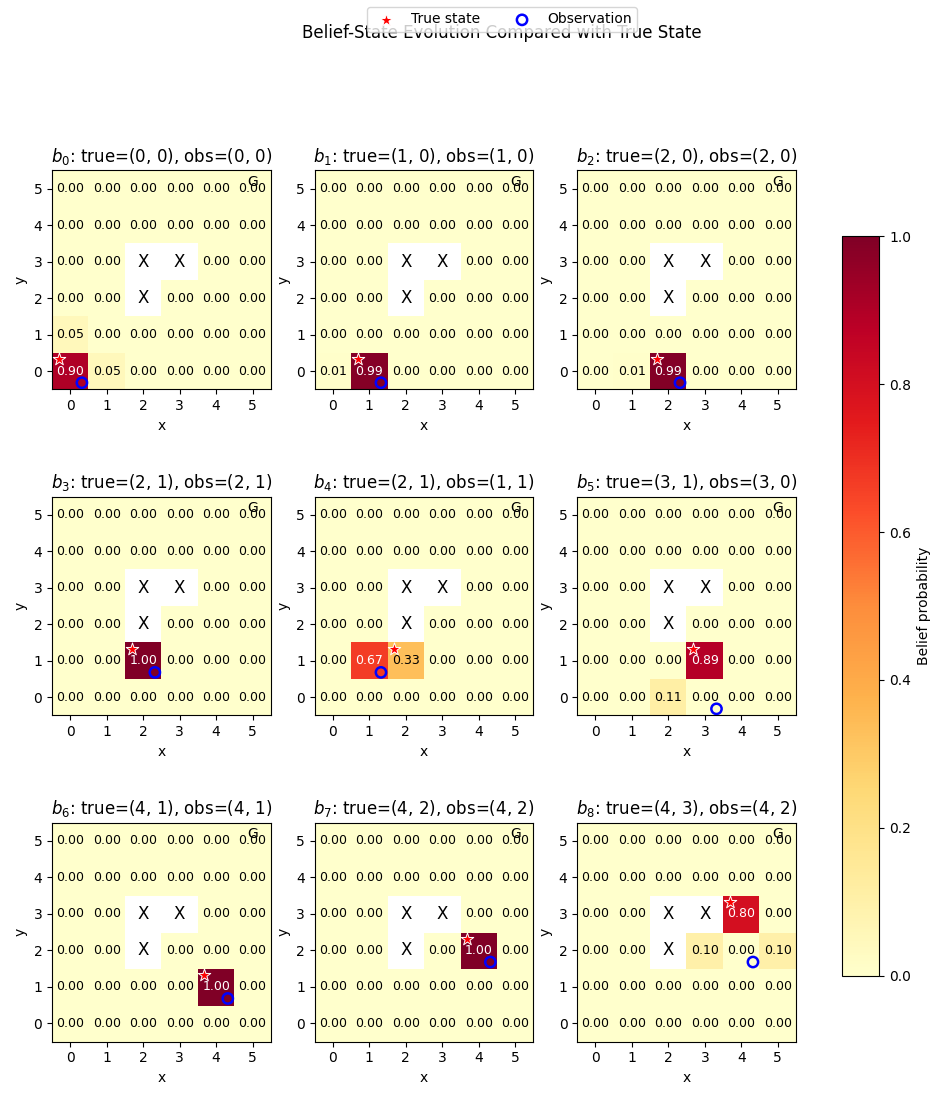
\includegraphics[height=0.79\textheight]{report_figures/2b.png}
  \caption{Belief-state evolution $b_0,\ldots,b_8$. The red star is the true state and the blue circle is the noisy observation. A common color scale is used across all nine panels.}
\end{figure}

The belief assigned to the true state at times $0$ through $8$ is, respectively,
\[
0.9000,\ 0.9856,\ 0.9918,\ 0.9995,\ 0.3333,\ 0.8889,\ 1.0000,\ 1.0000,\ 0.8000.
\]
The reductions at $t=4$, $t=5$, and $t=8$ correspond to deliberately noisy observations.

\subsection{3: MAP policy}

The MAP estimate is
\[
\hat x_t=\argmax_x b_t(x).
\]
The action treats $\hat x_t$ as the true state and minimizes its one-step MDP cost. The completed portion of \texttt{MAP.py} is:
\begin{lstlisting}
most_likely_state = np.argmax(belief)

best_action = np.argmin([
    stage_cost_c(most_likely_state, a)
    + sum([
        transition_prob[a, most_likely_state, s_next]
        * J_opt[t + 1, s_next]
        for s_next in range(S)
    ])
    for a in range(A)
])

return best_action
\end{lstlisting}

\subsection{4: QMDP policy}

The QMDP policy uses the entire belief distribution rather than only the most likely state. For each action, it computes
\[
\sum_x b_t(x)\left[c(x,u)+\sum_{x'}P(x'\mid x,u)J_{t+1}^*(x')\right]
\]
and chooses the action with the smallest belief-weighted expected cost. Intuitively, QMDP accounts for uncertainty in the robot's location instead of committing to a single estimated state.

\subsection{5: Policy performance}

Using 1,000 episodes per policy, start state $(0,0)$, and the provided seed $24$ gives:

\begin{table}[H]
\centering
\caption{MAP and QMDP performance under identical simulation settings.}
\begin{tabular}{lccc}
\toprule
Policy & Success rate & Average cumulative cost & Avg. time to goal\\
\midrule
MAP  & 0.925 & 13.085 & 11.714\\
QMDP & 0.941 & 12.774 & 11.694\\
\bottomrule
\end{tabular}
\end{table}

QMDP performs better in all three reported metrics in this experiment: it has a higher success rate, a lower average cumulative cost, and a slightly lower average time to the goal among successful runs.

The reason is that QMDP accounts for uncertainty in the current state rather than assuming that the most likely state is the only possible state. MAP can choose an action that is advantageous at its single most likely state but poor if the robot is actually in another state. This matters especially when the second most likely state has probability close to that of the MAP state.

One might initially expect MAP to reach the goal faster because it optimizes only for the most likely state. The results do not show that tradeoff here: QMDP's average successful-run time is smaller by $0.020$ steps. That difference is very small, so the experiment does not support a general claim that QMDP is inherently faster. It does show that QMDP is better on all three requested measures for this fixed setup and seed.

\section{Question 3: Discretization of a Convex Space}

Let $S=\operatorname{conv}\{s_1,\ldots,s_M\}$ and suppose $\widehat J_k$ is real-valued and convex over $S$. Recall that
\[
\widetilde J_k(x)=
\min\left\{
\sum_{i=1}^M\lambda_i\widehat J_k(s_i)
\ \middle|\
\sum_{i=1}^M\lambda_i s_i=x,\ 
\sum_{i=1}^M\lambda_i=1,\ 
\lambda_i\ge0
\right\},
\]
and
\[
\widehat J_k(x)=\min_{u\in U_k(x)}
\E\!\left[g_k(x,u,w_k)+
\widetilde J_{k+1}\bigl(f_k(x,u,w_k)\bigr)\right].
\]
Let $\mu_k$ be a policy attaining this latter minimum, and let $J_k$ be the actual cost-to-go when the policy sequence $\vec\mu$ is used.

\subsection{(a) Prove $\widehat J_k(x)\le\widetilde J_k(x)$}

Fix $x\in S$. Because $S$ is the convex hull of its finite subset $\widehat S=\{s_1,\ldots,s_M\}$, there is at least one feasible vector $\lambda$ such that
\[
x=\sum_{i=1}^M\lambda_i s_i,qquad
\sum_{i=1}^M\lambda_i=1,qquad \lambda_i\ge0.
\]
By the assumed convexity of $\widehat J_k$ and Jensen's inequality,
\[
\widehat J_k(x)
=\widehat J_k\!\left(\sum_{i=1}^M\lambda_i s_i\right)
\le \sum_{i=1}^M\lambda_i\widehat J_k(s_i).
\]
This holds for every feasible representation $\lambda$ of $x$, including a minimizing representation. Taking the minimum of the right-hand side over all feasible $\lambda$ yields
\answerbox{$\displaystyle
\widehat J_k(x)\le\widetilde J_k(x),
\qquad x\in S,\quad k=0,1,\ldots,N-1.$}

\subsection{(b) Prove $J_{N-1}(x)=\widehat J_{N-1}(x)\le\widetilde J_{N-1}(x)$}

At the terminal stage,
\[
J_N(x)=\widetilde J_N(x)=\widehat J_N(x)=g_N(x).
\]
Let $\bar u=\mu_{N-1}(x)$ denote the action selected by the one-step lookahead policy. From the definition of the actual policy cost-to-go,
\begin{align*}
J_{N-1}(x)
&=\E\!\left[
g_{N-1}(x,\bar u,w_{N-1})
+J_N\bigl(f_{N-1}(x,\bar u,w_{N-1})\bigr)
\right]\\
&=\E\!\left[
g_{N-1}(x,\bar u,w_{N-1})
+\widetilde J_N\bigl(f_{N-1}(x,\bar u,w_{N-1})\bigr)
\right].
\end{align*}
Because $\bar u=\mu_{N-1}(x)$ minimizes the last expression, its value is exactly the definition of $\widehat J_{N-1}(x)$. Thus
\[
J_{N-1}(x)=\widehat J_{N-1}(x).
\]
Part (a) gives $\widehat J_{N-1}(x)\le\widetilde J_{N-1}(x)$. Therefore,
\answerbox{$\displaystyle
J_{N-1}(x)=\widehat J_{N-1}(x)
\le\widetilde J_{N-1}(x),\qquad x\in S.$}

\subsection{(c) Prove $J_{N-2}(x)\le\widehat J_{N-2}(x)\le\widetilde J_{N-2}(x)$}

Let $\bar u=\mu_{N-2}(x)$. By the definition of the actual cost-to-go,
\begin{align*}
J_{N-2}(x)
&=\E\!\left[
g_{N-2}(x,\bar u,w_{N-2})
+J_{N-1}\bigl(f_{N-2}(x,\bar u,w_{N-2})\bigr)
\right].
\end{align*}
Part (b) states that $J_{N-1}(z)\le\widetilde J_{N-1}(z)$ for every $z\in S$. Applying this pointwise at the random next state and then taking expectations gives
\begin{align*}
J_{N-2}(x)
&\le\E\!\left[
g_{N-2}(x,\bar u,w_{N-2})
+\widetilde J_{N-1}\bigl(f_{N-2}(x,\bar u,w_{N-2})\bigr)
\right]\\
&=\min_{u\in U_{N-2}(x)}
\E\!\left[
g_{N-2}(x,u,w_{N-2})
+\widetilde J_{N-1}\bigl(f_{N-2}(x,u,w_{N-2})\bigr)
\right]\\
&=\widehat J_{N-2}(x),
\end{align*}
where the equality uses the fact that $\bar u=\mu_{N-2}(x)$ is the minimizing action. Finally, part (a) supplies the second inequality, so
\answerbox{$\displaystyle
J_{N-2}(x)\le\widehat J_{N-2}(x)
\le\widetilde J_{N-2}(x),\qquad x\in S.$}

\subsection{(d) Optional bonus: proof for every stage}

We use backward induction. At $k=N$, the terminal functions agree:
\[
J_N(x)=\widehat J_N(x)=\widetilde J_N(x)=g_N(x).
\]
Equivalently, part (b) establishes the first nonterminal base case at $k=N-1$.

Assume for some $k+1\le N-1$ that
\[
J_{k+1}(z)\le\widehat J_{k+1}(z)
\le\widetilde J_{k+1}(z)qquad\text{for every }z\in S.
\]
Let $\bar u=\mu_k(x)$. Then
\begin{align*}
J_k(x)
&=\E\!\left[
g_k(x,\bar u,w_k)
+J_{k+1}\bigl(f_k(x,\bar u,w_k)\bigr)
\right]\\
&\le\E\!\left[
g_k(x,\bar u,w_k)
+\widetilde J_{k+1}\bigl(f_k(x,\bar u,w_k)\bigr)
\right]\\
&=\min_{u\in U_k(x)}
\E\!\left[
g_k(x,u,w_k)
+\widetilde J_{k+1}\bigl(f_k(x,u,w_k)\bigr)
\right]\\
&=\widehat J_k(x).
\end{align*}
Part (a), which follows from convexity at every stage, gives
\[
\widehat J_k(x)\le\widetilde J_k(x).
\]
Thus the induction closes, proving
\answerbox{$\displaystyle
J_k(x)\le\widehat J_k(x)\le\widetilde J_k(x),
\qquad x\in S,\quad k=0,1,\ldots,N-1.$}

\end{document}
